%\documentclass[aps,preprint,nofootinbib,floatfix]{revtex4-1}
\documentclass{article}

%\usepackage{nips_2017}

% to compile a camera-ready version, add the [final] option, e.g.:
\usepackage[final]{nips_2017}

\usepackage{nicefrac}       % compact symbols for 1/2, etc.
\usepackage{microtype}      % microtypography
\usepackage{amsmath,amssymb,amsfonts,amsthm,amscd,bm,bbm}
\usepackage{algorithm}
\usepackage{algorithmic}
\usepackage[inline]{enumitem}

%\usepackage{cite}
\usepackage{bbm}
\usepackage{algorithm}
\usepackage{algorithmic}

\usepackage[pdftex]{graphicx}
\graphicspath{{./figs/}}

\hyphenation{op-tical net-works semi-conduc-tor}

\newtheorem{theorem}{Theorem}
\newtheorem{definition}[theorem]{Definition}
\newtheorem{assumption}[theorem]{Assumption}
\newtheorem{lemma}[theorem]{Lemma}
\newtheorem{corollary}[theorem]{Corollary}
\newtheorem{proposition}[theorem]{Proposition}
\newtheorem{conjecture}[theorem]{Conjecture}
\newtheorem{remark}[theorem]{Remark}
\newtheorem{example}{Example}

%% our definitions %%%%%%%%%%%%%%%%%%%%%%%%%%%%%%%%%%%%%%%%%%%%%%%%%%%%%%%%%%%%
\DeclareMathOperator{\aff}{aff}
\DeclareMathOperator{\st}{s.t.}
\DeclareMathOperator{\LC}{LC}
\DeclareMathOperator{\affnot}{aff_0}
\DeclareMathOperator{\conv}{conv}
\DeclareMathOperator{\relint}{relint}
\DeclareMathOperator{\vol}{vol}
\DeclareMathOperator{\range}{range}
\DeclareMathOperator{\image}{im}
\DeclareMathOperator{\nullspace}{null}
\DeclareMathOperator{\area}{area}
\DeclareMathOperator{\vspan}{span}
\DeclareMathOperator{\id}{Id}
\DeclareMathOperator{\cond}{cond}
\DeclareMathOperator{\prox}{prox}
\DeclareMathOperator*{\argmax}{arg\,max}
\DeclareMathOperator*{\argmin}{arg\,min}
\DeclareMathOperator*{\minimize}{minimize}
\DeclareMathOperator{\diag}{diag}
\DeclareMathOperator{\Tr}{Tr}

\newcommand\Energy{\mathcal{E}}
\newcommand\E{\mathbb{E}}
\newcommand\kk{K}
\newcommand\kkk{h}
\newcommand\Hk{{\mathcal{H}}_{\kk}}
\newcommand\HH{\mathcal{H}}
\newcommand\C{{\mathcal{C}}}
%\newcommand\Zt{\widetilde{Z}}
\newcommand\Zt{Y}
\newcommand{\Ind}[1]{\delta_{#1}}



\title{Nonparametric Clustering Based on Energy Statistics}

\author{
Guilherme Fran\c ca \\
Johns Hopkins University\\
\texttt{guifranca@gmail.com} \\
%% examples of more authors
\And
Joshua T. Vogelstein \\
Johns Hopkins University\\
\texttt{jovo@jhu.edu}
}


%\author{Guilherme Fran\c ca}
%\email{guifranca@gmail.com}
%\affiliation{Johns Hopkins University, Center for Imaging Science}

%\author{Joshua Vogelstein}
%\email{jovo@jhu.edu}
%\affiliation{Johns Hopkins University, Center for Imaging Science}

\begin{document}

\maketitle

\begin{abstract}
blabla
\end{abstract}



\section{Introduction}

Mention why energy is important, main results, where it was applied, etc.
Motivate how this can be used for clustering. Mention most important
papers on this \ldots Explain main results of this paper and give a brief
outline.


%%%%%%%%%%%%%%%%%%%%%%%%%%%%%%%%%%%%%%%%%%%%%%%%%%%%%%%%%%%%%%%%%%%%%%%%%%%%%%%
\section{Background on Energy Statistics and RKHS}
\label{sec:background}

In this section we briefly review the main concepts from energy
statistics and its relation to reproducing kernel Hilbert spaces 
(RKHS), which form the basis of our work.
For more details we refer the reader
to 
\cite{Szkely2013} 
(and references therein) and also \cite{Sejdinovic2013}.

Consider random variables in $\mathbb{R}^D$ 
such that $X,X' \stackrel{iid}{\sim} P$ and 
$Y,Y' \stackrel{iid}{\sim} Q$, where $P$ and $Q$ are cumulative
distribution functions with finite first moments. 
The quantity \cite{Szkely2013}
\begin{equation}\label{eq:energy}
\Energy(P, Q) = 2 \E \| X - Y\| - \E \| X - X' \| - \E \| Y - Y' \|,
\end{equation}
called \emph{energy distance}, 
is rotational invariant and nonnegative, $\Energy(P,Q) \ge 0$, where
equality
to zero holds if and only if $P = Q$.
Above, $\| \cdot \|$ denotes the
Euclidean norm in $\mathbb{R}^D$. 
Energy distance
provides a characterization of equality of distributions, and
$\Energy^{1/2}$ is
a metric on the space of distributions.

The energy distance can be generalized as, for instance,
\begin{equation}\label{eq:energy2}
\Energy_\alpha(P, Q) = 2 \E \| X - Y\|^{\alpha} - \E \| X - X' \|^{\alpha} - 
\E \| Y - Y' \|^{\alpha},
\end{equation}
where $0<\alpha\le 2$. This quantity is also nonnegative,
$\Energy_\alpha(P,Q) \ge 0$. Furthermore, for $0<\alpha<2$ we have that
$\Energy_\alpha(P,Q) = 0$ if and only if $P=Q$, while for $\alpha=2$ 
we have $\Energy_2(P,Q) = 2\| \E(X) - \E(Y) \|^2$, showing that
equality to zero only requires
equality of the means, and thus it does not imply equality of distributions.

It is important to 
mention that \eqref{eq:energy2} can be even further generalized.
Let $X, Y \in \mathcal{X}$ and replace the Euclidean norm by
$\rho: \mathcal{X}\times\mathcal{X} \to \mathbb{R}$, i.e.
$\| X - Y\| \to \rho(X,Y)$, where $\rho$ is a so-called \emph{semimetric
of negative type},
which satisfy 
\begin{equation}
\label{eq:negative_type}
\sum_{i,j=1}^n \alpha_i \alpha_j \rho(X_i, X_j) \le 0,
\end{equation}
where $X_i \in \mathcal{X}$, and $\alpha_i \in \mathbb{R}$ such that
$\sum_{i=1}^n \alpha_i = 0$.
In this case, there is a Hilbert space $\mathcal{H}$ and
a map $\varphi: \mathcal{X} \to
\mathcal{H}$ such that
$\rho(X, Y) = \| \varphi(X) - \varphi(Y) \|_{\mathcal{H}}^2$. 
Even though the semimetric 
$\rho$ may not satisfy the triangle inequality, 
$\rho^{1/2}$ does since it can be shown to be a legit metric. 

There is an equivalence between energy distance, 
commonly used in statistics,
and distances between embeddings of distributions in 
RKHS, commonly used in machine learning. 
This equivalence was established
in \cite{Sejdinovic2013}. Let us first recall the definition of
RKHS. Let $\HH$ be a Hilbert space of real-valued functions
over $\mathcal{X}$. A function 
$\kk : \mathcal{X} \times \mathcal{X} \to 
\mathbb{R}$ is a reproducing kernel of $\HH$ if it satisfies
the following two conditions:
\begin{enumerate}
\item $\kkk_x \equiv \kk(\cdot, x) \in \HH$ 
for any $x \in \mathcal{X}$.
\item $\langle \kkk_x, f \rangle_{\HH} = f(x)$ for
any $x\in\mathcal{X}$ and $f\in \HH$.
\end{enumerate}
In other words, for any $x \in \mathcal{X}$ there is a unique function
$\kkk_x \in \HH$ that reproduces $f(x)$ through the inner product
of $\HH$.
If such a \emph{kernel} 
function $\kk$ exists, then $\HH$ is called a RKHS.
From this we have $\langle \kkk_x, \kkk_y \rangle = \kkk_y(x) = \kk(x,y)$. 
This implies
that $\kk(x,y)$ is symmetric and positive semi-definite, 
$\sum_{i,j=1}^n c_i c_j
\kk(x_i,x_j) \ge 0$ for $c_i,c_j \in \mathbb{R}$.

The Moore-Aronszajn theorem establishes the converse \cite{Aronszajn}.
For every symmetric
and positive definite function $\kk: \mathcal{X}\times \mathcal{X} \to
\mathbb{R}$, there is an associated RKHS $\Hk$ 
with reproducing
kernel $\kk$. The map $\varphi: x \mapsto \kkk_x \in \Hk$ is called
the canonical feature map. Given a kernel $\kk$,
this theorem enables us to define an embedding of a probability measure
$P$ into the RKHS: $P \mapsto \kkk_P \in
\Hk$ such that 
$\int f(x) d P(x) = \langle f, \kkk_P \rangle$ for all $f \in \Hk$,
or alternatively $\kkk_P = \int \kk(\cdot, x)  d P(x)$. 
We can now  introduce the 
notion of distance between two probability measures using the inner product
of $\Hk$. This is called the maximum mean discrepancy (MMD) and
is given by
\begin{equation}\label{eq:mmd}
\gamma_\kk(P,Q) = \| \kkk_P - \kkk_Q \|_{\Hk},
\end{equation}
which can also be written as \cite{Gretton2012}
\begin{equation}\label{eq:mmd2}
\gamma_\kk^2(P,Q) = \E \kk(X,X') + \E \kk(Y,Y') - 2 \E \kk(X, Y)
\end{equation}
where $X,X' \stackrel{iid}{\sim} P$ and $Y,Y'\stackrel{iid}{\sim} Q$.
From the equality between \eqref{eq:mmd} and \eqref{eq:mmd2} we also
have 
\begin{equation}\label{eq:inner_data}
\langle \kkk_P, \kkk_Q \rangle_{\Hk} = \E \, \kk(X, Y).
\end{equation}
Therefore, in practice, we can estimate the inner product between the 
embedded distributions 
by averaging the kernel function over sampled data.

The following important result shows that semimetrics of negative
type and symmetric positive semi-definite kernels are closely related
\cite{Berg1984}. Let $\rho: \mathcal{X} \times \mathcal{X} \to \mathbb{R}$
be a semimetric, 
and $x_0 \in \mathcal{X}$ an arbitrary but fixed point.
Define
\begin{equation}
\label{eq:kernel_semimetric}
\kk(x,y) = \tfrac{1}{2} \left\{  \rho(x,x_0) + \rho(y,x_0) - \rho(x,y)\right\}.
\end{equation}
Then, $\kk$ is positive semi-definite if and only if $\rho$ is of negative type
\eqref{eq:negative_type}.
Here we have a family of kernels, one for each choice of $x_0$. Conversely,
if $\rho$ is a semimetric of negative type and $\kk$ is a kernel in this
family, then 
\begin{equation}
\label{eq:gen_kernel}
\rho(x,y) = \kk(x,x) + \kk(y,y) -2\kk(x,y) = \| \kkk_x - \kkk_y
\|^2_{\Hk},
\end{equation}
and the canonical feature map 
$\varphi: x \mapsto \kkk_x$ is injective \cite{Sejdinovic2013}.
We say that the kernel $\kk$ generates the semimetric $\rho$. 
If two different kernels generate the same $\rho$, they are
equivalent kernels.

Now we can state the equivalence between energy distance $\Energy$ and
inner products on RKHS, which is one of the main results of
\cite{Sejdinovic2013}. If $\rho$ is a semimetric
of negative type and $\kk$ a kernel that generates $\rho$, then
\begin{align}
\Energy(P, Q) &\equiv 2\E \, \rho(X,Y) - \E \, \rho(X,X') - \E \, \rho(Y,Y') 
\label{eq:EphoDef}\\
&= 2 \left[ \E \, \kk(X, X') + \E \, \kk(Y, Y') - 2\E \, \kk(X, Y)\right] \\
&=2 \gamma_\kk^2(P,Q) .
\end{align}
This result follows simply by substituting \eqref{eq:gen_kernel} into
\eqref{eq:EphoDef}, and using \eqref{eq:mmd2}.
Since $\gamma_k^2(P, Q) = \| \kkk_P - \kkk_Q \|^2_{\Hk}$ we
can compute the energy distance using the inner product of $\Hk$. Moreover,
this can be computed from the data according to \eqref{eq:inner_data}.

Finally, let us recall the main formulas for test statistics
\cite{Szkely2013}. 
Assume we have data $\mathbb{X} = \{ x_1,x_2,\dotsc, x_n \}$, where
$x_i \in \mathcal{X}$ is in some space of 
negative type \eqref{eq:negative_type},
and a partition $\mathbb{X} = \cup_{j=1}^k \C_j$ where
$\C_i \cap \C_j = \emptyset$.
Each expectation in 
\eqref{eq:EphoDef}
can be computed 
through the function
\begin{equation}
\label{eq:g_def}
g (\C_i, \C_j) \equiv 
\dfrac{1}{n_i n_j}
\sum_{x \in \C_i} 
\sum_{y \in \C_j} \rho(x, y)
\end{equation}
where $n_i = |\C_i|$ is the number of elements in 
$\C_i$. 
The \emph{within energy dispersion} is defined by
\begin{equation}
\label{eq:within}
W \equiv
\sum_{j=1}^{k} \dfrac{n_j}{2} g(\C_j, \C_j),
\end{equation}
and the \emph{between-sample energy statistic} is defined by
\begin{equation}
\label{eq:between}
S \equiv
\sum_{1 \le  j < l \le k } \dfrac{n_j n_{l}}{2 n} \left[
2 g(\C_j, \C_l) - 
g(\C_j, \C_j) - 
g(\C_l, \C_l)
\right].
\end{equation}
Given a set of distributions
$\{ P_j\}_{j=1}^k$ where $x \in \C_j \sim P_j$, the quantity
$S$ provides
a \emph{nonparametric} test statistic for equality of distributions.
Under the null hypothesis $H_0: P_1=P_2=\dotsm=P_k$, $S$ is small, 
and under
the alternative hypothesis $H_1: P_i \ne P_j$ for at least two $i\ne j$, 
$S \to \infty$ as the sample size is large, $n \to \infty$.
This test is nonparametric in the sense that it does not make any assumptions
about the distributions $P_j$.


%%%%%%%%%%%%%%%%%%%%%%%%%%%%%%%%%%%%%%%%%%%%%%%%%%%%%%%%%%%%%%%%%%%%%%%%%%%%%%%
\section{Clustering Based on Energy Statistics}
\label{sec:clustering_theory}

This section contains the main results of this paper, where 
we propose an optimization problem for clustering data
based on energy statistics and RKHS introduced in the previous section.

Based on the test statistic \eqref{eq:between}, the obvious
criterion for clustering data is to 
maximize $S$, which intuitivelly makes the distribution of each
cluster $\C_j$ as different
as possible from the other ones. However, the following 
simple result
shows that this is equivalent to minimizing
\eqref{eq:within}, which has a more convenient form.

\begin{proposition}
\label{th:minimize}
Let $\mathbb{X} = \{x_i\}_{i=1}^{n}$ where 
$x_i$ lives in a space $\mathcal{X}$ endowed with a semi-metric $\rho$ of
negative type. For a fixed integer $k$,
the partition
$\mathbb{X} = \cup_{j=1}^k \C_j$, where $\C_i \cap C_j = \emptyset$ for
all $i\ne j$, maximizes $S$ if and only if
\begin{equation}
\label{eq:minimize}
\min_{\{ \C_j \} } W(\{ 
\C_1, \dotsc, \C_k
\}).
\end{equation}
\end{proposition}
\begin{proof}
It can be shown that the total dispersion of the data obeys \cite{Szkely2013}
\begin{equation}
W + S = \dfrac{n}{2} g(\mathbb{X}, \mathbb{X}). 
\end{equation}
Note, however, that the right hand side of this equation 
only depends on the pooled data, so it is a constant
independent on the choice of partition. Therefore, maximizing
$S$ is equivalent to minimizing~$W$.
\end{proof}

Thus, given $k$, our clustering problem ammounts to
finding the best partition of the data through solving~\eqref{eq:minimize}.
In this setting, each datapoint belongs to one and only one cluster
(hard assignments).

Based on 
\eqref{eq:kernel_semimetric} and \eqref{eq:gen_kernel}, assume that 
the kernel $\kk: \mathcal{X} \times \mathcal{X} \to \mathbb{R}$ 
generates $\rho$. 
Let us define  the kernel matrix
$G \in \mathbb{R}^{n\times n}$ such that
\begin{equation}
\label{eq:kernel_matrix}
G_{ij} \equiv \kk(x_i, x_j).
\end{equation}
Let $Z$ be the label matrix, $Z \in \{ 0,1 \}^{n\times k}$, 
with only one nonvanishing entry per row indicating to which cluster (columns)
each point (rows) belongs to. This matrix satisfy
$Z^\top Z = D$ where $D = \diag( n_1,\dotsc, n_k )$  contains
the number of points in each cluster. We also introduce the rescaled
matrix  $Y \equiv Z D^{-1/2}$. In component form they are given by
\begin{equation}
\label{eq:label_matrix}
Z_{ij} \equiv \begin{cases}
1 & \mbox{if $x_i \in \C_j$ } \\
0 & \mbox{otherwise}
\end{cases} \qquad
\Zt_{ij} \equiv \begin{cases}
\tfrac{1}{\sqrt{n_j}} & \mbox{if $x_i \in \C_j$ } \\
0 & \mbox{otherwise}
\end{cases} .
\end{equation}

Our next result reveals the optimization problem behind \eqref{eq:minimize},
which is in general NP-hard since
it is a quadratically constrained quadratic problem (QCQP).

\begin{proposition} 
\label{th:qcqp2}
The problem \eqref{eq:minimize} is equivalent to
\begin{equation}
\label{eq:qcqp2}
\max_{\Zt} \Tr \left\{ \Zt^\top G \Zt \right\}  \qquad
\mbox{s.t. $\Zt \ge 0$, $\Zt^\top \Zt = I$, 
$\Zt \Zt^\top \bm{e} = \bm{e}$},
\end{equation}
where $\bm{e} = (1,1,\dots,1)^\top \in \mathbb{R}^n$ is the all-ones vector,
and $G$ is the pairwise kernel matrix \eqref{eq:kernel_matrix}, assumed
to be given.
\end{proposition}
\begin{proof}
Replacing \eqref{eq:gen_kernel}  into
\eqref{eq:g_def},  
we can write \eqref{eq:within} as
\begin{equation}
\label{eq:W2}
W(\{ \C_j \} )
= \dfrac{1}{2} \sum_{j=1}^k \dfrac{1}{n_j} \sum_{x,y \in \C_j} \rho(x,y)
= \sum_{j=1}^k \sum_{x \in \C_j}  \bigg(
\kk(x,x) - \dfrac{1}{n_j} \sum_{y \in \C_j} \kk(x,y) \bigg).
\end{equation}
The first term is a global constant 
which does not contribute,
so minimizing \eqref{eq:W2} is the same as
\begin{equation}
\label{eq:max_prob}
\max_{ \{ \C_j \} } \sum_{j=1}^k \dfrac{1}{n_j} \sum_{x,y\in C_j} \kk(x,y) .
\end{equation}
But 
\begin{equation}
\sum_{x, y \in \C_j} \kk(x, y) =
\sum_{l=1}^{n} \sum_{m=1}^{n} Z_{lj} Z_{mj} G_{lm} = 
(Z^\top G Z)_{jj}
\end{equation}
where we used the definitions \eqref{eq:kernel_matrix} and
\eqref{eq:label_matrix}. Thus \eqref{eq:max_prob} is equal to
$\max \Tr \left\{ D^{-1} Z^\top G Z \right\}$. Now we can
use the cyclic property
of the trace, and by the own definition of the matrix $Z$
in \eqref{eq:label_matrix} we obtain the following integer
programing problem:
\begin{equation}\label{eq:qcqp}
\begin{aligned}
& \max_{Z} \Tr\left\{ \big( Z D^{-1/2}\big)^\top G 
\big( ZD^{-1/2} \big) 
\right\} \\
&\mbox{s.t. $Z_{ij} \in \{0,1\}$, $\sum_{j=1}^k Z_{ij} = 1$, 
$\sum_{i=1}^n Z_{ij} = n_j$.}
\end{aligned}
\end{equation}
Now we write this in terms of $Y = Z D^{-1/2}$, given by
\eqref{eq:label_matrix}. The objective function immediately becomes
$\Tr Y^\top G Y$. Notice that the above constraints
immediatly imply that $Z^T Z = D$, which in turn gives
$D^{-1/2} Y^T Y D^{-1/2} = D$, or $Y^\top Y = I$. 
Also, every entry of $Y$ is positive by definition,
$Y \ge 0$. Now it only remains to show the last 
constraint in \eqref{eq:qcqp2}, which comes from the last
constraint in \eqref{eq:qcqp}. In matrix form this reads
$Z^T \bm{e} = D \bm{e}$. Replacing by $Z=YD^{1/2}$ we have
$Y^\top \bm{e} = D^{1/2} \bm{e}$. Multiplying this last equation
on the left by $Y$, and noticing
that $Y D^{1/2} \bm{e} = Z \bm{e} = \bm{e}$, we finally obtain
$Y Y^\top \bm{e} = \bm{e}$ as desired.
\end{proof}

Therefore, to cluster data $\{ x_i \}_{i=1}^n \in \mathcal{X}$ into 
$k$ partitions,
assuming that $k$ is given, we first compute the kernel matrix
$G$  --- 
which is  defined by an arbitrary semimetric of negative 
type on $\mathcal{X}$  --- and then 
solve the optimization problem \eqref{eq:qcqp2} for $\Zt \in
\mathbb{R}^{n\times k}$. The $i$th row
of $\Zt$ will contain a single nonzero element in some $j$th column,
indicating that $x_i \in \C_j$.

In general, 
problem \eqref{eq:qcqp2} is NP-hard and there
are few methods
available to tackle this kind of problem directly,
which is computational prohibitive even for relatively small datasets.
However, one can find an approximate solution by relaxing some 
of the constraints, or obtaining a relaxed SDP version of it. 
For instance, a simple approximation can be given
by 
$\max_{Y} \Tr Y^\top G \, Y $ subject to $Y^\top Y = I$,
and requiring that the rows of $Y$ are normalized. 
It is possible to find a global solution to this problem by
choosing $Y$ as the top $k$ eigenvectors of $G$, which results
in 
$\max \Tr \left\{ Y^\top G \, Y \right\}  = \sum_{i=1}^k \lambda_i(G)$, 
which is the
sum of the top $k$ eigenvalues of $G$. This is what is usually done
in spectral clustering. However, we will propose a simple iterative
algorithm in the next section.

An interesting point is that \eqref{eq:qcqp2} has the same
formulation as kernel $k$-means, spectral clustering, and the maximum
cut problem on graphs \cite{Dhillon}. 
Proposition~\ref{th:qcqp2} brings energy statistics based clustering
into this broad picture, and \eqref{eq:qcqp2} should have 
interesting applications in
graph partitioning problems and unsupervised learning in general.
Notice that it is straightforward to generalize \eqref{eq:qcqp2} to
a weighted version, where weights $W = \diag(w(x_1), \dotsc, w(x_n))^\top $
are associated to each data point $x_i$. One just replace the objective
function in \eqref{eq:qcqp2} by 
\begin{equation}
\max_Y \Tr \left\{ Y^\top W^{1/2} G W^{1/2} Y \right\}.
\end{equation}
Furthermore, and most importantly, our analysis is valid
for any space $\mathcal{X}$ equiped with a semimetric of negative type $\rho$.
This method is
nonparametric since it does not assume any form of the 
distribution of the data,
contrary to $k$-means and gaussian mixture models (GMM), for example.
Moreover, this approach does not require the concept of the cluster mean, or
median, which can be ill-defined in some types of data, such as images for
instance.


%%%%%%%%%%%%%%%%%%%%%%%%%%%%%%%%%%%%%%%%%%%%%%%%%%%%%%%%%%%%%%%%%%%%%%%%%%%%%%%
\section{A Simple Iterative Algorithm}
\label{sec:iterative_algo}

We can formulate an iterative algorithm to find
an approximate solution to \eqref{eq:qcqp2} on the same lines
as kernel $k$-means.
Let $t$ be the iteration time. First precompute the kernel
matrix $G$, fix the number of clusters $k$, then
perform the following steps:
\begin{enumerate}
\item \label{initialize} 
Initialize clusters $\{ \C_1^{(0)},\dotsc,\C_k^{(0)} \}$, which
determines the label matrix $\Zt^{(0)}$.
\item \label{assignment} For each datapoint $x_i$ compute
its cluster assignment through
\begin{equation}
\label{eq:algo}
\Zt^{(t+1)}_{ij} = 
\begin{cases}
\tfrac{1}{\sqrt{n_j}} & \mbox{if $j = \argmax_\ell \tfrac{1}{n_\ell} 
\sum_{m=1}^n G_{i m} \Zt^{(t)}_{m\ell}$ } \\
0 & \mbox{otherwise.}
\end{cases}
\nonumber
\end{equation}
\item If converged return $\Zt^{(t+1)}$, otherwise
set $t = t+1$ and repeat step~\ref{assignment}.
\end{enumerate}
If data is $D$-dimensional, computing $G$ has complexity
$O(n^2 D)$. Step \ref{assignment} above has complexity $O(n)$ for
each point, thus total complexity $O(n^2)$. Assuming we perform $T$ 
iterations,
the total complexity of the algorithm is $O(n^2(D + T))$.
We can initialize the algorithm in step~\ref{initialize} with any method
we want, a good alternative is the initialization from $k$-means++.


%%%%%%%%%%%%%%%%%%%%%%%%%%%%%%%%%%%%%%%%%%%%%%%%%%%%%%%%%%%%%%%%%%%%%%%%%%%%%%%
\section{Two-Class Problem in One Dimension}

Here we consider an alternative approach in the simplest case possible, which
is one-dimensional data and a two-class problem.
If we choose
$\rho(x,y) = |x - y|$, we can actually compute 
\eqref{eq:g_def} in $O(n \log n)$ instead of $O(n^2 D)$ and find
a direct solution to \eqref{eq:minimize}. 
This is done by noticing that
\begin{equation}
\begin{aligned}
|x - y|  &= \Ind{x \ge y} (x - y) -
\Ind{x < y} (x - y) \\
&= 
\left( \Ind{x \ge y} - \Ind{x < y} \right) x + 
\left( \Ind{y > x} - \Ind{y \le x} \right) y
\end{aligned}
\end{equation}
where $\Ind{}$ is the indicator function.
Let $\C$ be a partition with
$n$ elements. Using the above distance in \eqref{eq:g_def} we have
\begin{equation}
\label{eq:g_ind}
g(\C,\C) = \dfrac{1}{n^2} \sum_{x \in \C} 
\sum_{y \in \C} 
\left(
\Ind{x \ge y} + \Ind{y > x} - 
\Ind{x \ge y}-\Ind{x < y} \right) x.
\end{equation}
The sum over $y$ can be eliminated since the term in
parenthesis is simply counting the number of elements in $\C$ that satisfy
the conditions of the indicator functions. Therefore, assume
that we order the data as 
$\bar{\C} = [ x_j \in \C: x_1 \le x_2 \le \dotsm \le x_{n}]$. Thus, we
can write \eqref{eq:g_ind} in the following very simple form:
\begin{equation}
\label{eq:g1d}
g(\C, \C) = \dfrac{2}{n^2} \sum_{\ell=1}^n (2\ell - 1 - n) x_\ell .
\end{equation}
Note that the cost of computing this is $O(n)$, once the data
is sorted which costs at the most $O(n\log n)$.
Now suppose we order each partition, obtaining $\mathbb{X} = \cup_{j=1}^k
\bar{\C}_j$. Then \eqref{eq:within} is given by
\begin{equation}
\label{eq:w1d}
W(\{ \bar{\C}_i \}) = 
\sum_{j=1}^k \sum_{\ell=1}^{n_j} \dfrac{2\ell - 1 - n_j}{n_j} \, x_\ell.
\end{equation}
For a two-class problem, we can cluster the data by computing \eqref{eq:w1d}
for each possible split, and pick the one with minimum value. This is done
as follows:
\begin{enumerate}
\item Sort the pooled data, obtaining the sorted set $\bar{\mathbb{X}}$ with
$n$ elements.
\item For each $t=1,2,\dotsc,n$, make two partitions 
$\bar{\C}_1^{(t)} = [x_i]_{i=1}^t$ and 
$\bar{\C}_2^{(t)} = [x_i]_{i=t+1}^n$. 
\item Compute $W^{(t)} = W(\{ \bar{\C}_1^{(t)},\bar{\C}_2^{(t)}  \})$ 
from \eqref{eq:w1d}.
\item The best split is $t^\star = \argmin_t W^{(t)}$, which
determines the final clusters.
\end{enumerate}
Notice that this procedure does not require any initialization, however,
it only works for one-dimensional data and for Euclidean distance.


\section{Numerical Experiments}


\begin{figure}
\begin{minipage}{0.33\textwidth}
\centering
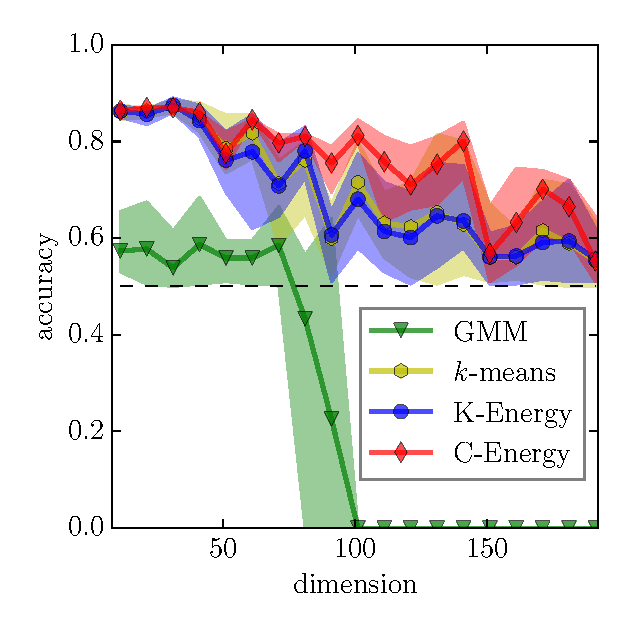
\includegraphics[width=\textwidth]{gauss_means.pdf}\\[-.8em]
(a)
\end{minipage}
\begin{minipage}{0.33\textwidth}
\centering
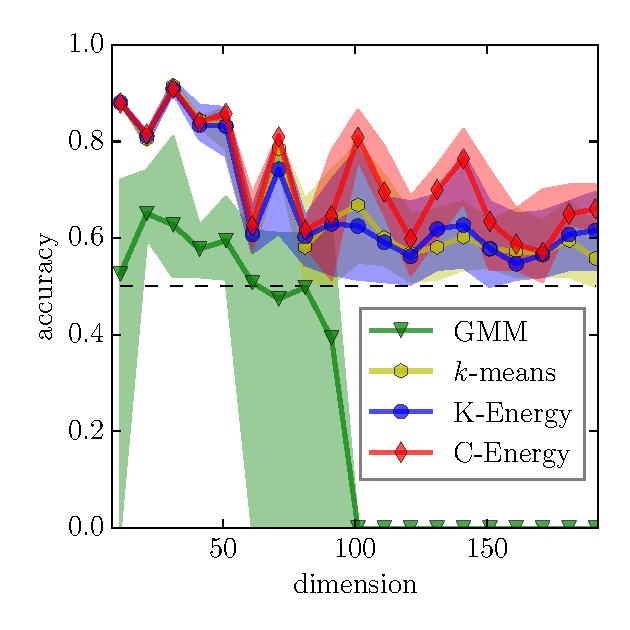
\includegraphics[width=\textwidth]{gauss_covs.pdf}\\[-.8em]
(b)
\end{minipage}
\begin{minipage}{0.33\textwidth}
\centering
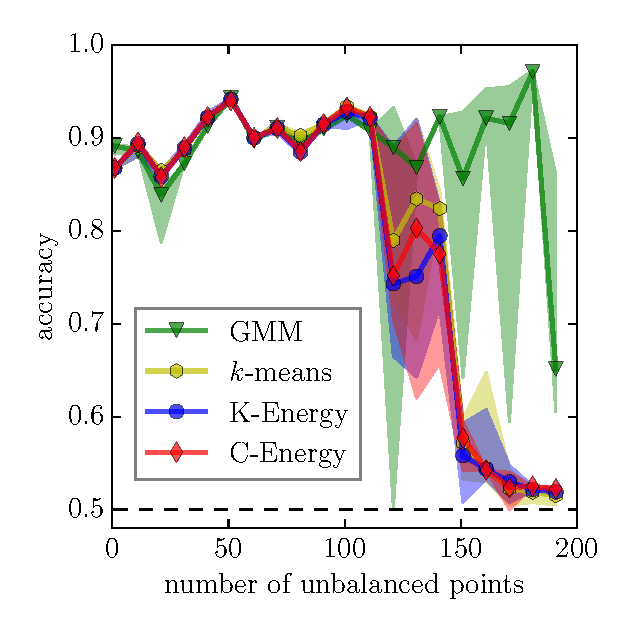
\includegraphics[width=\textwidth]{gauss_pis.pdf}\\[-.8em]
(c)
\end{minipage}
\caption{
\label{fig:dimension}
gadsga
}
\end{figure}

\begin{figure}
\centering
\caption{
\label{fig:unbalanced}
gadsga
}
\end{figure}

\begin{figure}
\begin{minipage}{0.33\textwidth}
\hspace{.7cm}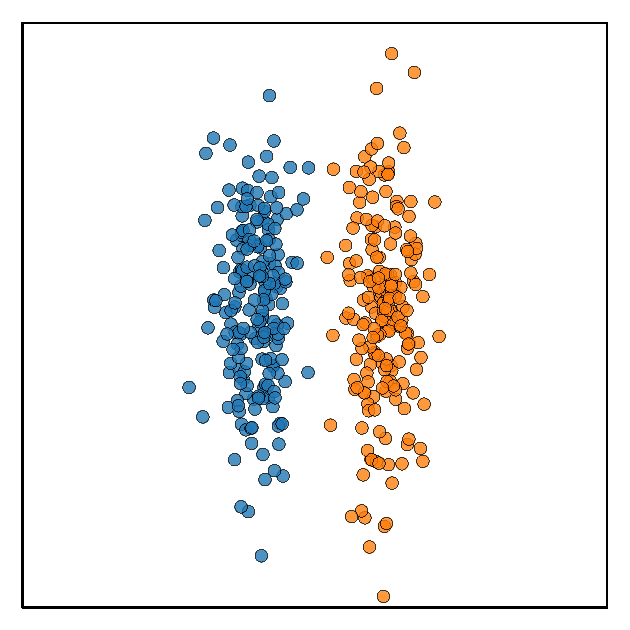
\includegraphics[width=.82\textwidth]{cigar_data.pdf}
\end{minipage}
\begin{minipage}{0.33\textwidth}
\hspace{.7cm}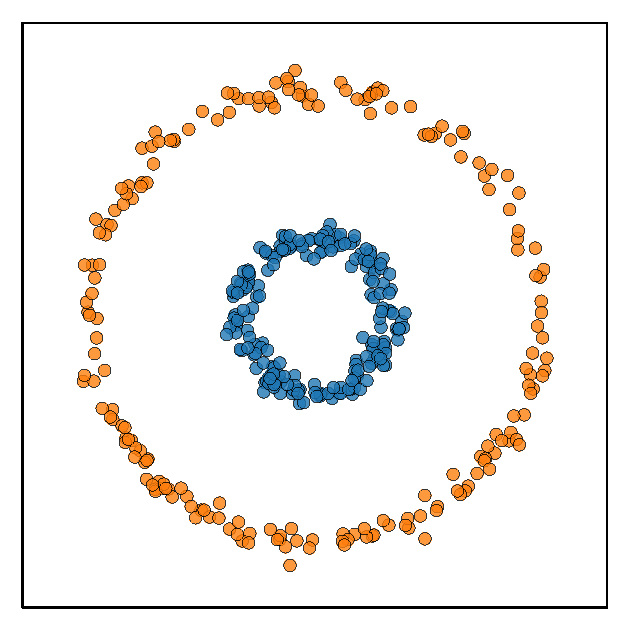
\includegraphics[width=.82\textwidth]{circles_data.pdf}
\end{minipage}
\begin{minipage}{0.33\textwidth}
\hspace{.7cm}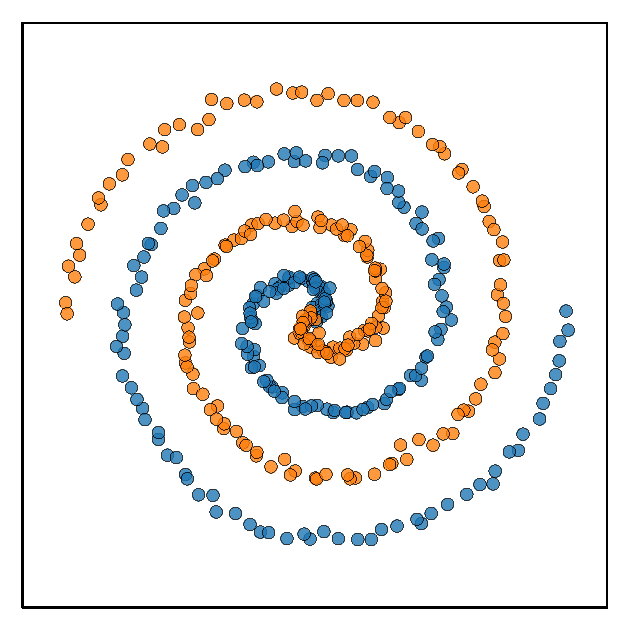
\includegraphics[width=.82\textwidth]{spirals_data.pdf}
\end{minipage}
\begin{minipage}{0.33\textwidth}
\centering
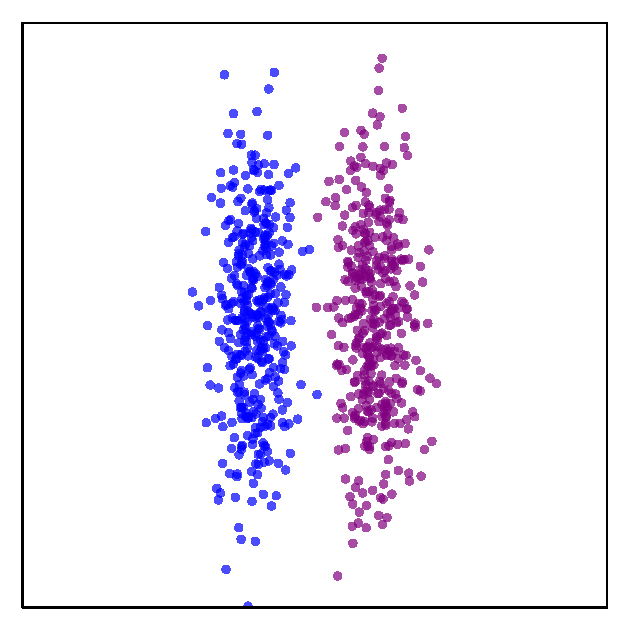
\includegraphics[width=\textwidth]{cigars.pdf}\\[-.8em]
(a)
\end{minipage}
\begin{minipage}{0.33\textwidth}
\centering
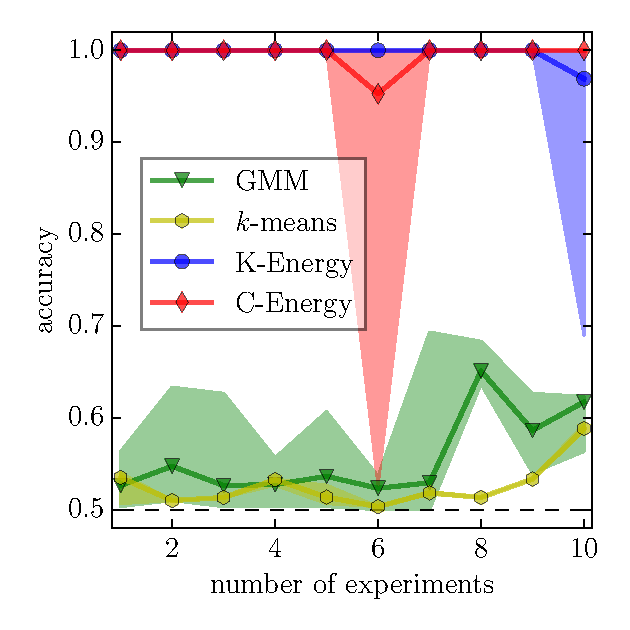
\includegraphics[width=\textwidth]{circles.pdf}\\[-.8em]
(b)
\end{minipage}
\begin{minipage}{0.33\textwidth}
\centering
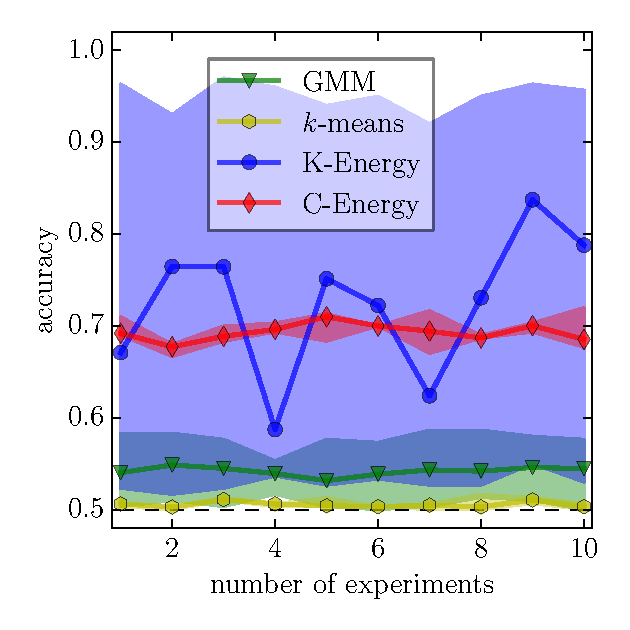
\includegraphics[width=\textwidth]{spirals.pdf}\\[-.8em]
(c)
\end{minipage}
\caption{
\label{fig:dimension}
gadsga
}
\end{figure}


\section{Conclusion}


\subsection*{Acknowledgements}
We thank \ldots


\bibliographystyle{unsrt}
\bibliography{biblio.bib}



\end{document}
